\documentclass[acmtog]{acmart}
\usepackage{graphicx}
\usepackage{subfigure}
\usepackage{natbib}
\usepackage{listings}
\usepackage{bm}
\usepackage{amsmath}

\definecolor{blve}{rgb}{0.3372549 , 0.61176471, 0.83921569}
\definecolor{gr33n}{rgb}{0.29019608, 0.7372549, 0.64705882}
\makeatletter
\lst@InstallKeywords k{class}{classstyle}\slshape{classstyle}{}ld
\makeatother
\lstset{language=C++,
	basicstyle=\ttfamily,
	keywordstyle=\color{blve}\ttfamily,
	stringstyle=\color{red}\ttfamily,
	commentstyle=\color{magenta}\ttfamily,
	morecomment=[l][\color{magenta}]{\#},
	classstyle = \bfseries\color{gr33n}, 
	tabsize=2
}
\lstset{basicstyle=\ttfamily}

% Title portion
\title{Assignment 2:\\ {Assignment 2 : Geometric Modeling}} 

\author{Name:\quad ZhouShouchen  \\ student number:\ 2021533042
\\email:\quad zhoushch@shanghaitech.edu.cn}
\setlength{\headheight}{25pt}


% Document starts
\begin{document}
\maketitle

\vspace*{2 ex}

\section{Introduction}
In this assignment, the following tasks are finished by using OpenGL.
\begin{itemize}
\item Task1: use the basic iterative de Casteljau Bézier vertex evaluation algorithm to get the Bézier curve.
\item Task2: construct the Bézier surface.
\item Task3: render a Bézier Surface in a OpenGL window.
\item Task4: stitch multiple Bézier surface patches together.
\item Bonus1: Adaptive mesh construction in parameter space based on the curvature estimation.
\item Bonus2: B-Spline surface construction. 
\item Bonus3: Interactive editing (by selection) of control points.

\end{itemize}
\section{Implementation Details}

\subsection{evaluate Bézier curve}
we use $t$ as the paramater ranged at $[0,1]$ to control the Bézier curve.\\
a Bézier curve with degree $n$ is decided by $n+1$ control points $P_i$.\\
the basic defination of the Bézier curve is that \\$B(t)=\sum_{i=0}^n \binom{n}{i}(1-t)^{n-i}t^iP_i$\\
but throw this method, it may lead to trouble to calculate the combination number, and it is had to get the normal vector at each point on Bézier curve.\\
so we use de Casteljau Bézier vertex evaluation algorithm to recursively evaluate the curve,
the method is two find two connected points, and calculate a new point throw $P\_new=(1-t)*P_i+t*P_{i+1}$,
P are the points, and i is the index.\\
and for the last two points, their connection direction is the normal vector's direction at the last point for each $t$.

\subsection{evaluate Bézier surface}
$\vec{P}(u,v)=\sum_{i=0}^n\sum_{j=0}^mB_i^n(u)B_j^m(v)\cdot\vec{k_{i,j}}$\\
where $k_{i,j}$ is the control point with the index of $(i,j)$\\
however, it might be kind of complex, so we can use the similar method with Bézier curve.\\
we use paramaters $u,v$ ranged at $[0,1]*[0,1]$ to control the Bézier surface.\\
\begin{itemize}
\item firstly, along the u direction, we can have $n$ Bézier curves, each curve has $m$ control points.
with paramater u, we can access $n$ new control points.
After that, we use these new control points to get another Bézier curve, and get the 
final point with $v$.\\
after these options, we can get the point with index $(u,v)$ and its tangent vector on the direction of $v$.\\

\item similarly, along the v direction, we can have $m$ Bézier curves, each curve has $n$ control points.
with paramater v, we can access $m$ new control points.
After that, we use these new control points to get another Bézier curve, and get the 
final point with $u$.\\
after these options, we can get the point with index $(u,v)$ and its tangent vector on the direction of $u$.\\

\end{itemize}

and it is clear that the two points we get above have the same position, but 
different targent. To get the normal vector $\vec{m}$ which is vertical to the plane.

$\vec{m}$ needs to be vertical to both targant along direction u and v,
to figure out this, we just need a cross product

let $\vec{m}=normalize(\frac{\partial \vec{P}}{\partial u} \times \frac{\partial \vec{P}}{\partial v})$\\
actually, we do not need to write it twice to get a Bézier surface, during the next subsection, 
we just need to two swap the control points' $n,m$ index, and swap $u,v$ , to call the function twice is 
much more convenience.

\subsection{render Bézier surface}
\begin{itemize}
	\item to initialize a object class, we need to bind $VAO,VBO,VEO(EBO)$ same as what we did in assignment 1.
	\item and we need to observe datas, the main method of loading data are in next subsection.
	\item for shaders, we can just use the phong lightning model to help us render the objects.
\end{itemize}
when rending the mesh, we can first evaluate some points of the Bézier surface through de Casteljau's algorithm with the control of given contrl points.\\
and for each points, connect his adjacent points to form a triangle, and the we can just send the triangles to the vertex shader, and then rending the surface.

\subsection{stitch multiple Bézier surface patches}
in the main fuction, we need to call the $read$ funciotn to open file in $assets$, but the code and the $.bzs$ file are in different
folders, so we can use $../assets/tea.bz$ to load the file.\\
for each file, it contains $b$ surfaces' control points, with total $p$ points, each Bézier surface have $m\cdot n$ control points.
after infile, we use class $BezierSurface$ to save the data.\\
and we should stitching multiple Bézier surface patches together to create a complex meshes.\\
1st order continuity (L1) means that not only the points are connected, but also their tangents (first derivative) are continuous at the joint. To ensure this, we need to make sure that the control polygon are colinear at the last control point of the first curve/surface and the first control point of the second curve/surface.\\
to make it smooth, the control points at the two side of the connection, these three points should be in the 
same line, and they are equally spaced.\\ 
however, the nice data has already helped us to satisfy this condition, which means that the connected faces
shared the same control points, so the stitching of connected surfaces' tangents (first derivative) are continuous at the joint.\\
So the surface after stitching still looks smooth.

\subsection{Adaptive mesh construction}
the task can be devided into two parts,
the adaptive mesh construction and the triangulation.\\
because after the adaptive mesh construction, the mesh is no longer a rectangular texure mapping, it become irregular.\\
so the triangulation is needed.
\begin{itemize}
\item adaptive mesh construction
Using static sampling steps may cause precision loss.
We can sample the curve adaptively by considering curvature of sampled points to achieve a better effect.

\item trianglation
we can use the Delauny Triangulation.\\
the algorithm is like:\\
while(there exists illegal edge $p_ip_j$)\{\\
\ \ \ assume there are two neighbor traingle $p_ip_jp_k$ and $p_ip_jp_l$\\
\ \ \ replace $p_ip_j$ by $p_kp_l$\\
\}\\
and the illegal edge is that the inscribed circle of that edge contains other trangle's vertex, then the edge is illegal. 
\end{itemize}

Due to time limit, a better effect is not achieved. I deeply regret about this.

\subsection{B-spline surface}
The biggest advantage of B-spline surface over Bezier surface is local modification\\
B-spline algorithm is that the whole curve is connected by one segment of curve, and it is generated by piecewise continuous multi-segment.\\
from the defination of the B-spline surface,suppose that p is the surface,\\
and mark that the degree of the basis function is k. The ith k-th B-spline basis function is $B_{i,k}(u)$\\
$p(u,v)=\sum_{i=0}^m\sum_{j=0}^n B_{i,p}(u)B_{j,q}(v)P_{i,j}$\\
where $B_{i,p}(u),B_{j,q}(v)$ are the basic function,\\
and $P_{i,j}$ are $(m+1)*(n+1)$ control points.\\
and the basic function's defination is :\\
$B_{i,0}(u)= 1, u_i \leq u < u_{i+1}, i=0,1,...,m-1$
$B_{i,0}(u)= 0, otherwise$
$B_{i,k}(u) = \frac{u-u_i}{u_{i+k}-u_i}B_{i,k-1}(u)+\frac{u_{i+k+1}-u}{u_{i+k+1}-u_{i+1}}B_{i+1,k-1}(u)$
and other operations are similar with the Bézier surface,
and for the normal vector, we can use a small interpolation the replace the targent vector, later use cross product to get the normal vector.\\
similarly with Bézier surface, we can recursively use the de Boor's algorithm which is similar with de Casteljau's algorithm.\\
and for details, we need to set a sequence of knots, and a degree is needed, the degree must be less than the number of control points of a B-spline curve.\\
and we can uniform subdivision 0.0 to 1.0, and set more degree number of 0.0 at the beginning, and more degree number of 1.0 in the end.\\
with these initializations, we can use de Boor's algorithm to solve out the B-spline surface.

\subsection{interactive}
\begin{itemize}
	\item principle 
	to get the mouse's world space's position, we just need to get the inverse way that we get the clip space's position.\\
	since $V_{clip}=M_{projection}\cdot M_{view}\cdot M_{model}\cdot V_{local}$\\
	so space position \\$V_{world}=M_{model}\cdot V_{local}= M_{view}^{-1}\cdot M_{projection}^{-1}\cdot V_{clip}$\\
	however, the OpenGL's shader has helped us to change the positions from clip space into the screen space, 
	so before using the formulas above, we need to change the mouse's position from screen space into the clip space first.\\
	the steps are as followed:
	\begin{itemize}
		\item get normalized device from normalized screen at focus point depth ([0,1])\\
		let $ ndcCoords = ((2 * mouse\_x - WIDTH) / WIDTH, (2 * mouse\_y - HEIGHT) / HEIGHT, -0.1f)$\\
		the $mouse\_x,mouse\_y$ is the mouse's position on the screen space,
		and the $WIDTH,HEIGHT$ are the size of the screen window.
		\item get clip pos from normalized device coords\\
		let $clipW = projection[2][3] / $\\$(ndcCoords.z - (projection[2][2] / projection[3][2]))$\\
		$ clipCoords = vec4(ndcCoords * clipW, clipW)$\\
		$projection$ is the projection matrix mentioned above, and the index of matrix of OpenGL is different from the matrix we used, it is more like a transpose.
		\item get world pos from normalized device coords\\
		let $eyeCoords = glm::inverse(projection) * clipCoords$\\
		$worldCoords = glm::inverse(view) * eyeCoords$\\
		$worldCoords /= worldCoords.w$\\
		$mouse_world = vec3(worldCoords)$\\
		what's more, the y-axis in the world space is opposite from the screen space,\\
		so we need to let $mouse\_world.y = -mouse\_world.y$
		\item judge whether the mouse and the control point is in the same place of screen space
		we can just judge in the world space: whether the control point is on the line of the camera's position and the mouse's position on the near plane. let the line be $\vec{vecb}$.\\	
		to judge this, we can get two vectors, $\vec{veca}$ is the line of the camera's position and the control point.\\
		the the distance of the control point and the $\vec{vecb}$ is $\frac{\left| \vec{veca} \times \vec{vecb} \right|}{\left| \vec{vecb} \right|}$
		\item move the control point with the mouse
		since the mouse and the control point are in the same line at the begin, so at that time we can get the ratio,\\
		which is ratio of the distance of their positions and the camera's position.
		every time the mouse moved, we can calculate the control point's pose by times the ratio with mouse's position.
	\end{itemize}


	\item operation mode
	at the beginning, all blue balls symbolized a control point.\\ 
	when the mouse is near a control point in screen space, the ball representing the control point turns red.\\
	to move that control point, we just need to click the mouse's right bottom, and then the control point turns into green, and its directions are shown(x,y,z-axis)\\
	after that, the control point will move with the mouse, to stop moving, we just need to click the right bottom of the mouse,
	then the control points will stop moving, and turns into blue again.\\
	the Bézier surface will change immediately when the control points are moving.
\end{itemize}


\section{Results}
% pictures should be in
the results can be seen in the pictures.

\begin{itemize}
	\item Fig. 1. As it is shown, we stitch multiple Bézier surface patches together,
	and it seems smooth at the connection place from all different directions. The light uses the phong lightning model. 
	
	\item Fig. 2. for the first two image, they are some surface controled by some points made by myself.\\
	and the blue ball on the image are the control points.\\
	the last $4$ images are using the data of the $tea.bzs$ which was used in the first part, the data to draw Bézier surface.\\
	since the Bézier are drawn by a series of $4 \times 4$ control points. So the degree to draw the B-spline surface must be $\leq 3$.
	so for the last $4$ images, it is a comparation.\\
	the third image is of $degree=1$\\
	the fourth image is of $degree=2$\\
	the fifth image is of $degree=3$\\
	and the last image is a Bézier surface for comparation.\\
	it seems that the uniform samplingB-spline surface of degree=3 looks similar with the Bézier surface.

	\item Fig. 3. As it is shown, all control points are symbolized as a ball colored blue, we the mouse is near to a control point,
	it turns to blue.\\
	And when we want to move the control point, with clicking the left bottom, it turned to green. And axises are printed.\\
	after moving, click the right bottom, and it turns blue again.\\ 
	the Bézier surface change with the control points' changing.
	
	\end{itemize}

\begin{figure}[h]
	\centering
	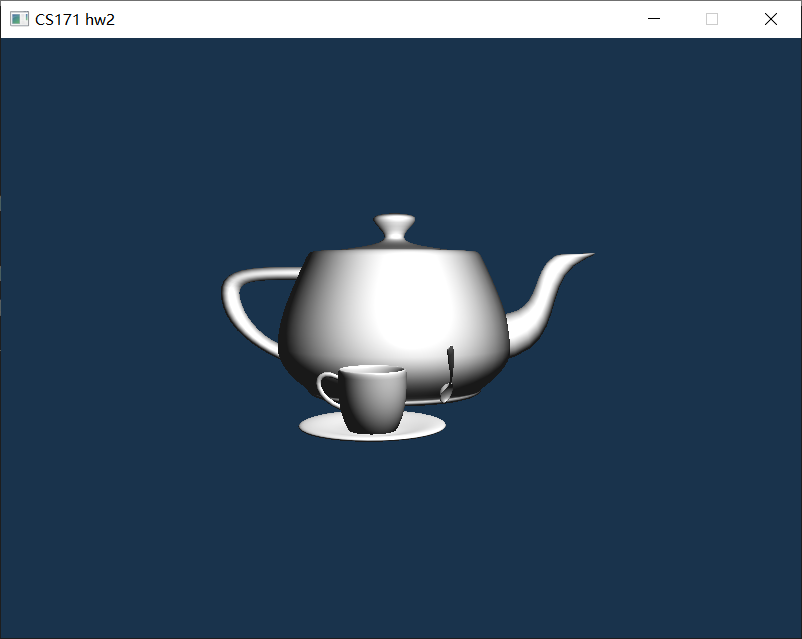
\includegraphics[width=4cm,height=5cm]{1}
	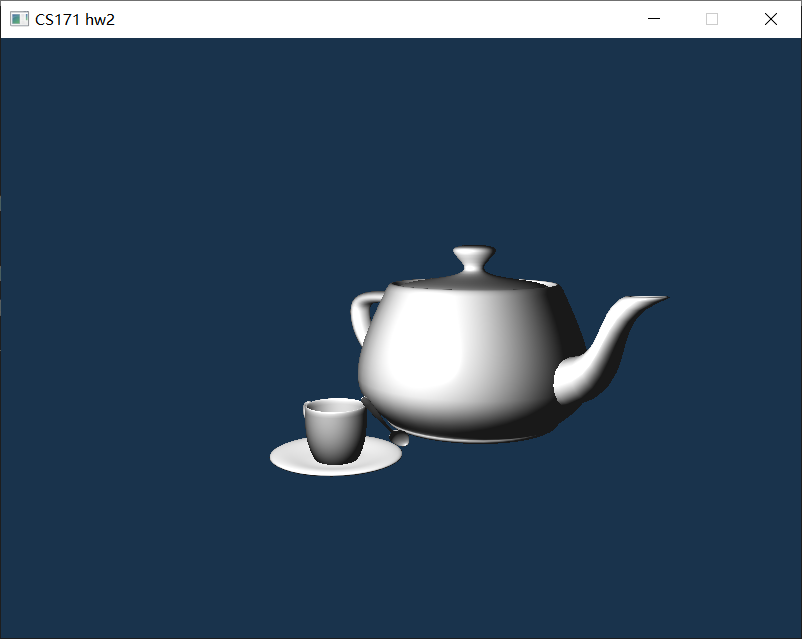
\includegraphics[width=4cm,height=5cm]{2}
	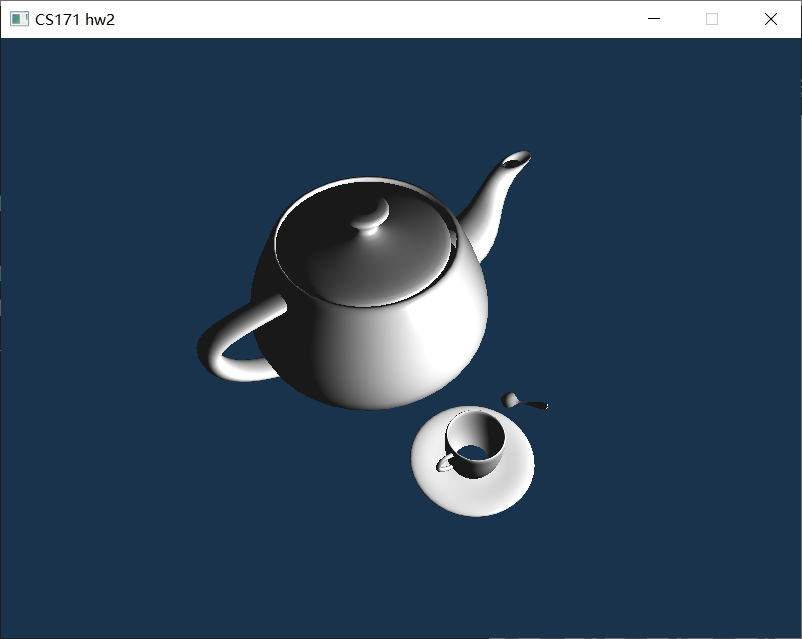
\includegraphics[width=4cm,height=5cm]{3}
	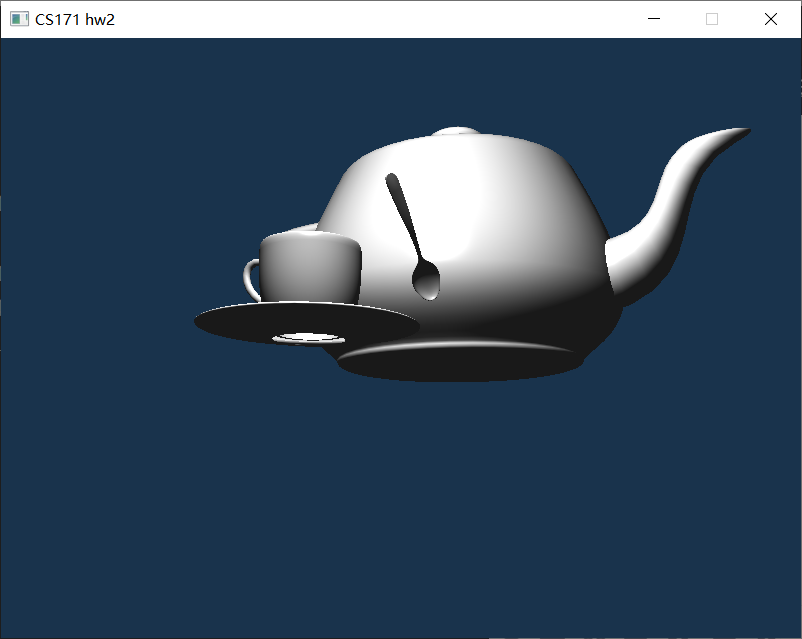
\includegraphics[width=4cm,height=5cm]{4}
	\caption{the tea party from different directions}
\end{figure}


\begin{figure}[h]
	\centering
	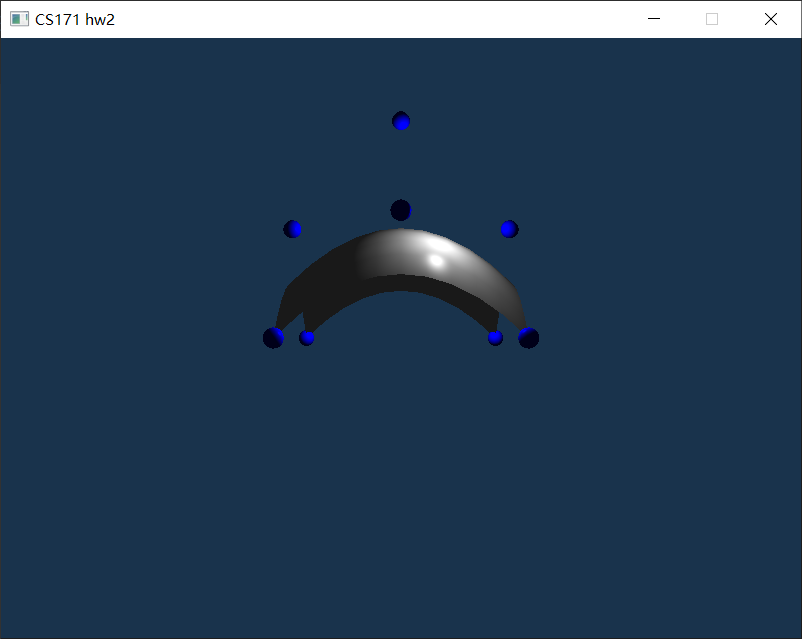
\includegraphics[width=4cm,height=5cm]{bspline1}
	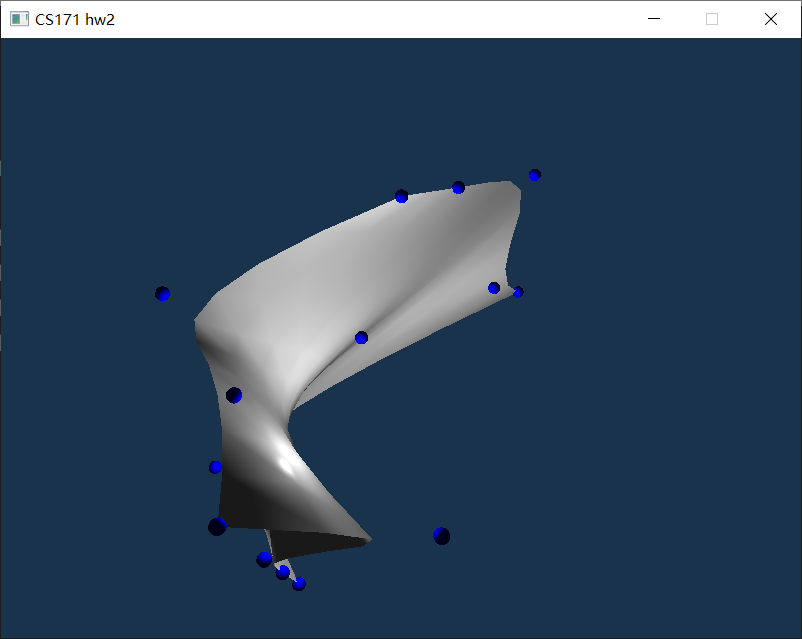
\includegraphics[width=4cm,height=5cm]{bspline2}
	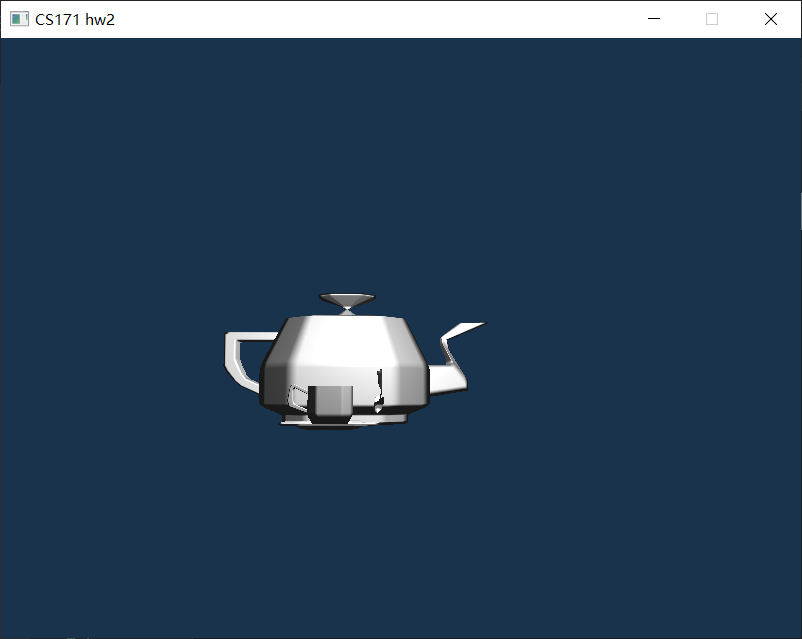
\includegraphics[width=4cm,height=5cm]{degree1}
	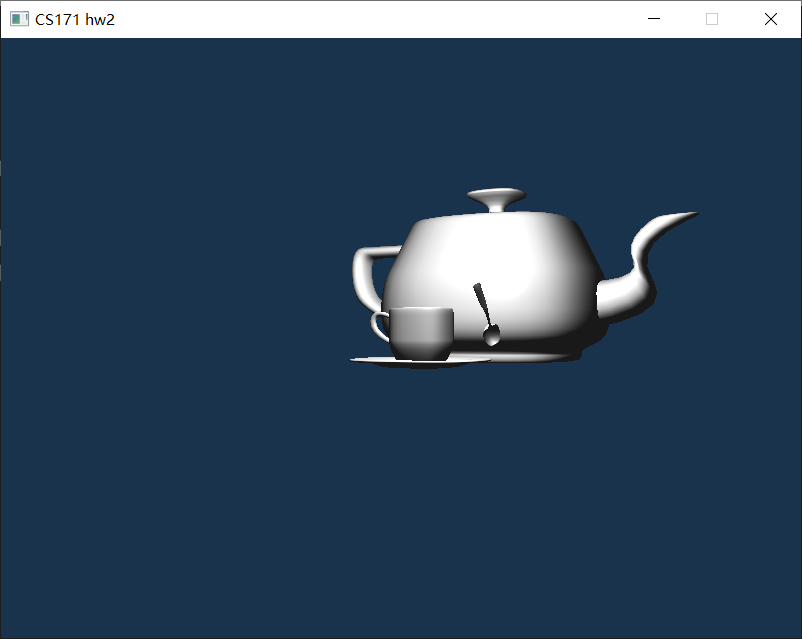
\includegraphics[width=4cm,height=5cm]{degree2}
	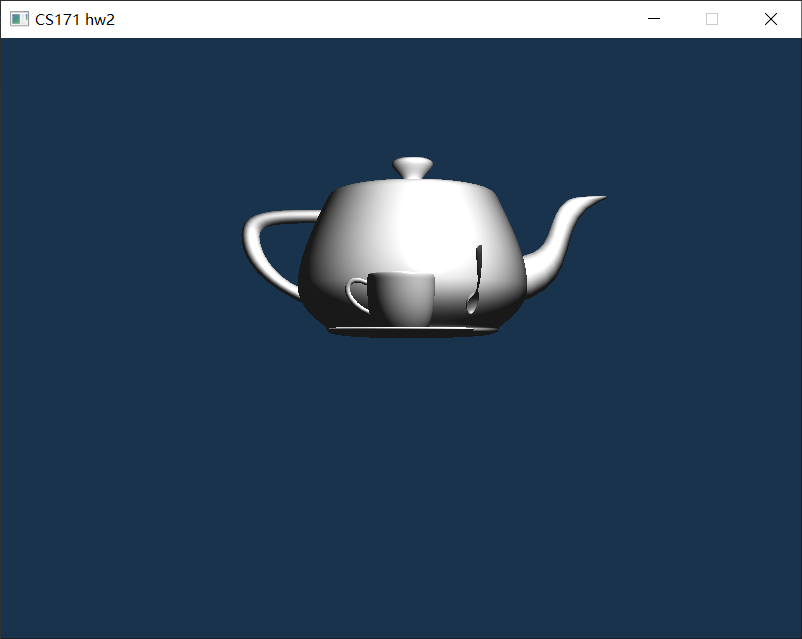
\includegraphics[width=4cm,height=5cm]{degree3}
	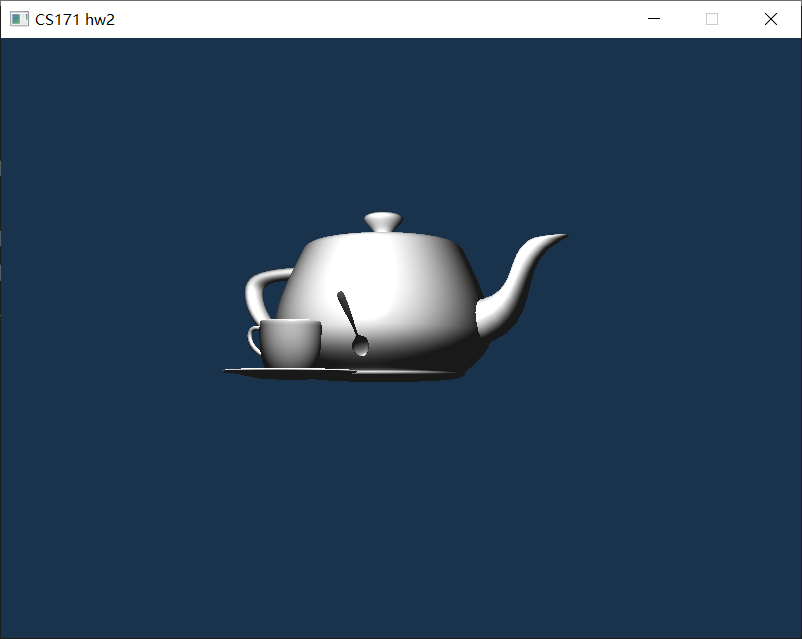
\includegraphics[width=4cm,height=5cm]{bezier}
	\caption{some surface using Bspline to draw}
\end{figure}


\begin{figure}[h]
	\centering
	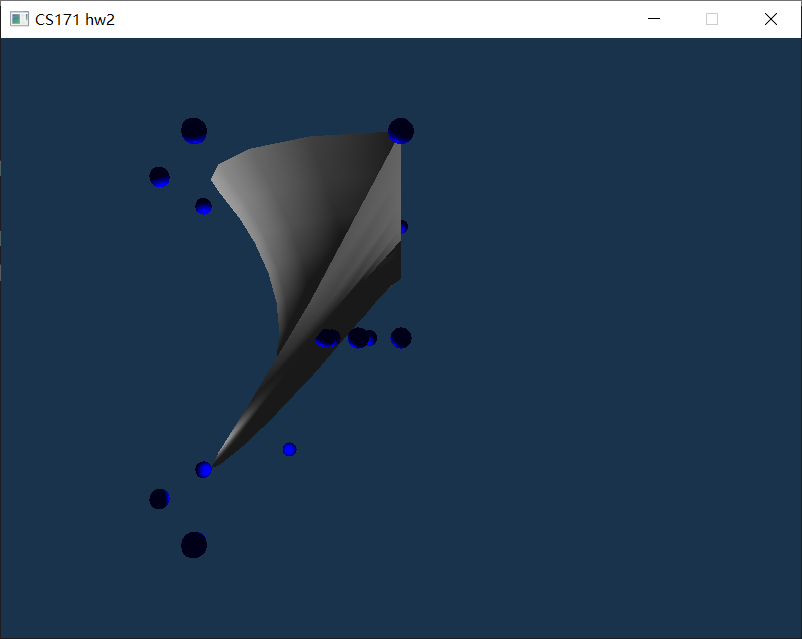
\includegraphics[width=4cm,height=5cm]{inter1}
	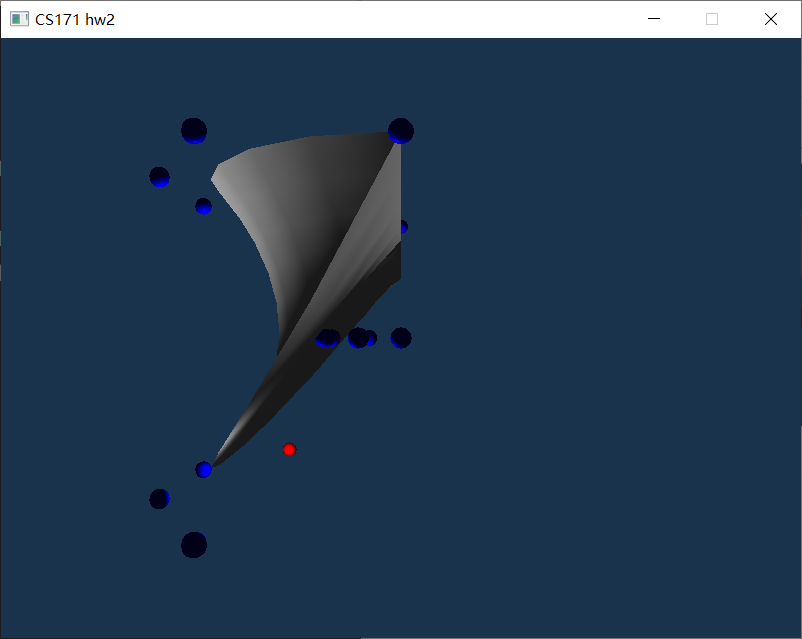
\includegraphics[width=4cm,height=5cm]{inter2}
	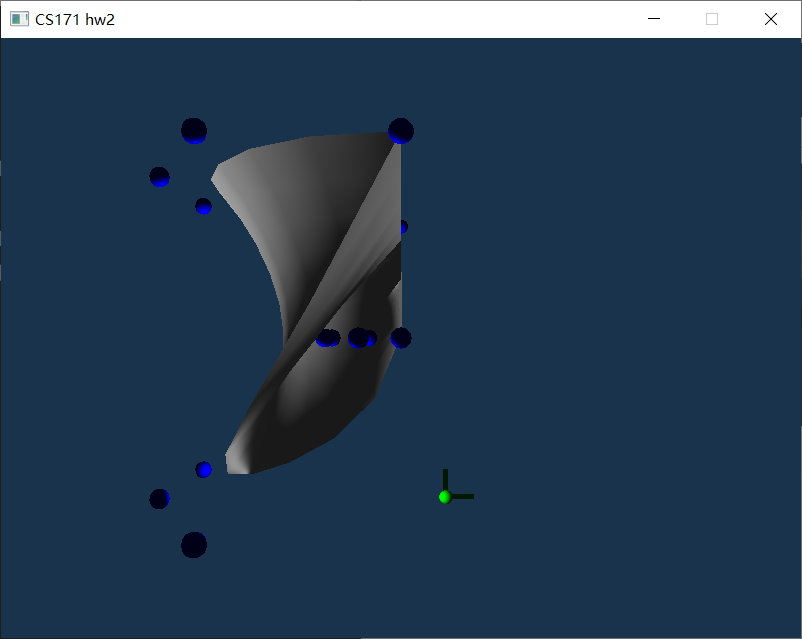
\includegraphics[width=4cm,height=5cm]{inter3}
	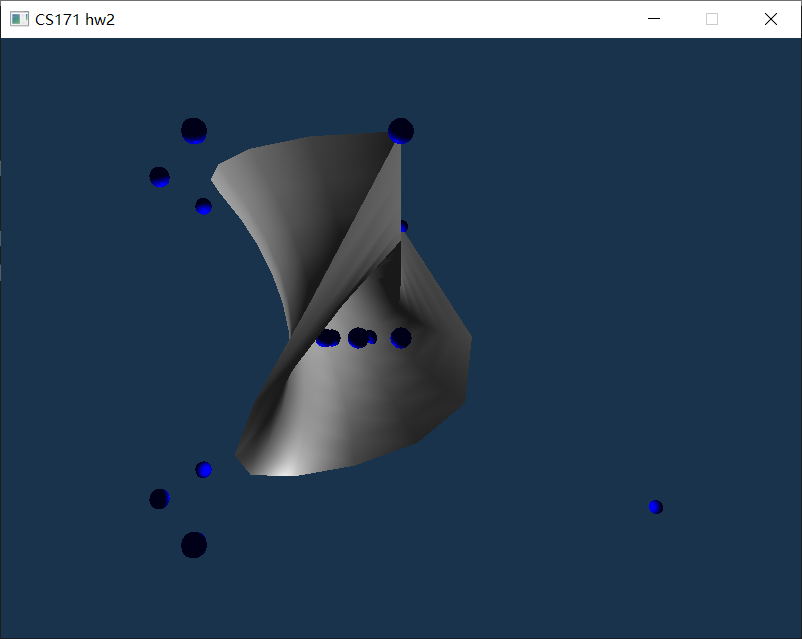
\includegraphics[width=4cm,height=5cm]{inter4}
	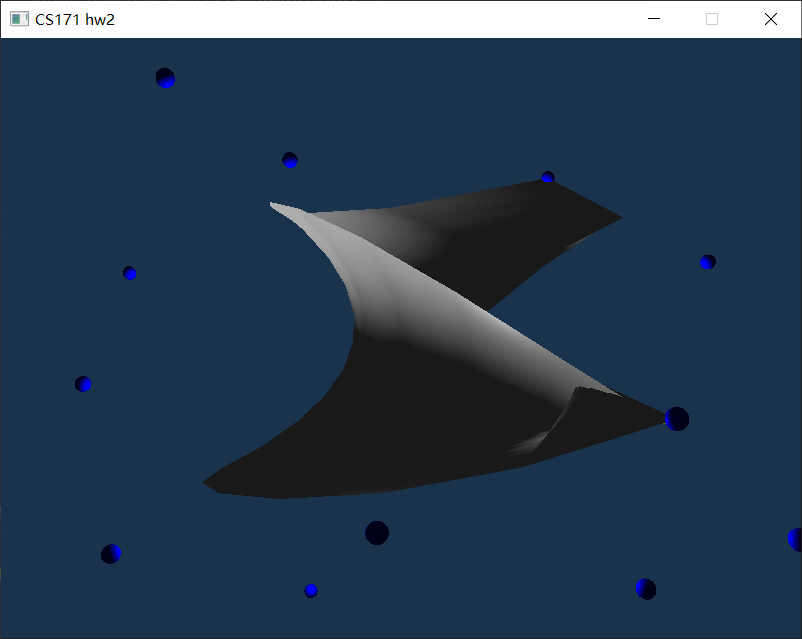
\includegraphics[width=4cm,height=5cm]{inter5}
	\caption{Interactive editing of control points}
\end{figure}

.
\\
\end{document}
